\chapter{Augmented Reality (AR)}
\label{cha:ar}

When we speak about AR, we mostly think about overlaying or adding information to the real world. In most cases this happens with the help of a head-mounted device that contains a see through display. If the display is completely opaque and shields the users view from the reality, we speak about Virtual Reality (VR). \newline
Even though it may seem like AR is a relatively new technology, the idea of it can be traced back to more than 100 years ago, way before the first computer. Back then, the american author L. Frank Baum, famous for his book ``The Wonderful Wizard of Oz'', described a device that can be compared to modern AR glasses. In his short story ``The Master Key'' from 1901, he writes about a pair of electrical glasses that show the wearer the character of the person in front of him in form of a letter over their head~\cite{baum96}. It took almost another 70 years until Ivan E. Sutherland proposed his idea of a head-mounted display in his paper from 1968~\cite{sutherland68}.
And even though many people think about head-mounted displays~\cite{milgram94} when they hear about AR, it is not limited to glass-like devices. As long as some computer generated graphics are merged with the real world and are shown to the user, we can speak about Augmented or even Mixed Reality (MR). 


\section{Use Cases}
AR can be used in many different situations, however, not all of them are suitable for everyday use. That is also because the hardware for more advanced displaying has to be good and is therefore still in the upper price range and hardly affordable for normal users. Furthermore, many devices are still quite big or have a limited battery capacity. Here are some usages:
\begin{description}
	\item[Information overlay]  
	Information overlay is one of the easiest use cases, however it is still a very useful technique. The idea is that users, wearing the AR glasses or holding their smartphone, are getting information about their surroundings. A good example for that is Google Lens, an application that scans and interprets whatever is filmed with the phone's camera. The software can scan things or text, to look it up online~\cite{patel18}, give style ideas~\cite{schaefer19} or be a tour guide in an unfamiliar city~\cite{malczyk19}. Apps that run on head-mounted devices can be advantageous, for example when driving a motorcycle or bike to give information about speed, directions, or even have a 360 degree field of view with the help of additional cameras. \newline
	The overlay is mostly non-immersive, meaning that the users do not feel like they are in a virtual  world. The artifacts simply get displayed in front of the eyes or on any other display, preferably not obstructing anything else. Even in the car, a projection of information like road conditions, speed, directions or other useful information can be an area of application~\cite{wayray}.
	\item[Translation]
	A case where it is useful for the generated graphics to overlay things in the real world, is when AR is used for translation, like provided by Google Translate~\cite{gu19}. The application uses text recognition to detect writing in a picture or video stream coming from a camera and translates it. The translation is then displayed directly over the real world text, so that the users just see text that they can understand. That can be useful while driving in a foreign country to quickly and directly understand street signs. A slightly modified approach is to use a microphone instead of a camera and use speech recognition to hear and translate the words to show the user.
	\item[Instructions]
	What we want to do and what many AR glasses are used for, is giving instructions and showing the users what they have to do. A popular use case is giving the users directions on how to assemble a machine that they are not familiar with or, like Antifakos et al.~\cite{antifakos02} did, give instructions on how to build furniture. In that way users can have clearly shown instructions that are integrated with the real world. Ideally they are shown on a head-up display (HUD) so that the user does not have to look away from his work and also has his or her hands free for work.
	\newpage
	\item[Computer Games]
	Gaming is one of the smaller fields, since here the usage of VR seems to be preferred by bigger game studios. AR is mostly used on phones with the help of the camera to simulate transparency and interacting with the real life. The advantage of games on smartphones is that nowadays the computing power often is better than on glasses. A famous one is Pokemon Go~\cite{pokemongo} from 2014, played on the smartphone. Here the phone camera and screen is used to show the real life, overlayed with graphics from the game. 
	\item[Room planning/designing]
	There are applications, among others from IKEA \cite{ikea17}, that let you design your interior with the help of AR. They simply work on your smartphone and let you insert models of their furniture into your living room, with the help of the camera. Everything works in real time with nothing more than a smartphone. 
	\item[Architecture/Construction]
	AR can be used in many ways for showing users buildings and constructions that do not exist yet. It can help to give a better understanding on how something like a house should or will be build and can even give workers a plan on what the architect has envisioned. Delgado et al.~\cite{delgado20} researched in their article, how augmented reality can be used in architecture, engineering and construction and found various ways on how it can be used in the process of building, for stakeholder engagement, design support, construction support or even training.
	One possible way of using AR in the field of archaeology is to use it for visualization of reconstructed sights. Dähne and Karigiannis~\cite{daehne02} proposed a system to virtually rebuild ruins at historical sites and give the user a tour. AR provides visual input on how the buildings could have looked like. 
	\item[TV]
	One of the most consumed form of AR is utilized in television every day. Many TV stations want to spice up their weather forecast and show the viewer a moving and changing map with the weather showing and the presenter interacting with it. That can go from simple symbols up to fully displayed tornadoes or floods in the studio like done by IBM Max Reality~\cite{ibm}, seen on Figure~\ref{fig:ibm_mr},  all just to entertain the viewers. Similar methods are used when showing statistical data, for example the results of votes in different parts of the country, like ORF, national television in Austria, did it at the 2019 Austrian legislative election, seen in Figure \ref{fig:election}. 
	Pejman et al.~\cite{pejman19} even tried to add AR artifacts to the existing TV program to give viewers additional content and tested it on a documentary.
	
	
	
	\begin{figure}[!ht]
		\captionsetup{justification=centering}
		\centering
		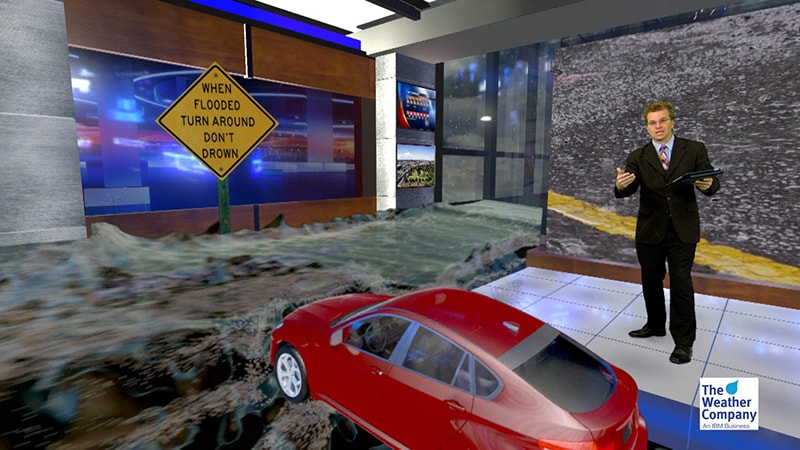
\includegraphics[width=0.78\textwidth]{media/ibm_max_reality.jpg}
		\hfill
		\caption{Flooding in the studio, made possible by IBM Max Reality, taken from~\cite{ibm}.}
		\label{fig:ibm_mr}
	\end{figure}
	\begin{figure}[!ht]
		\captionsetup{justification=centering}
		\centering
		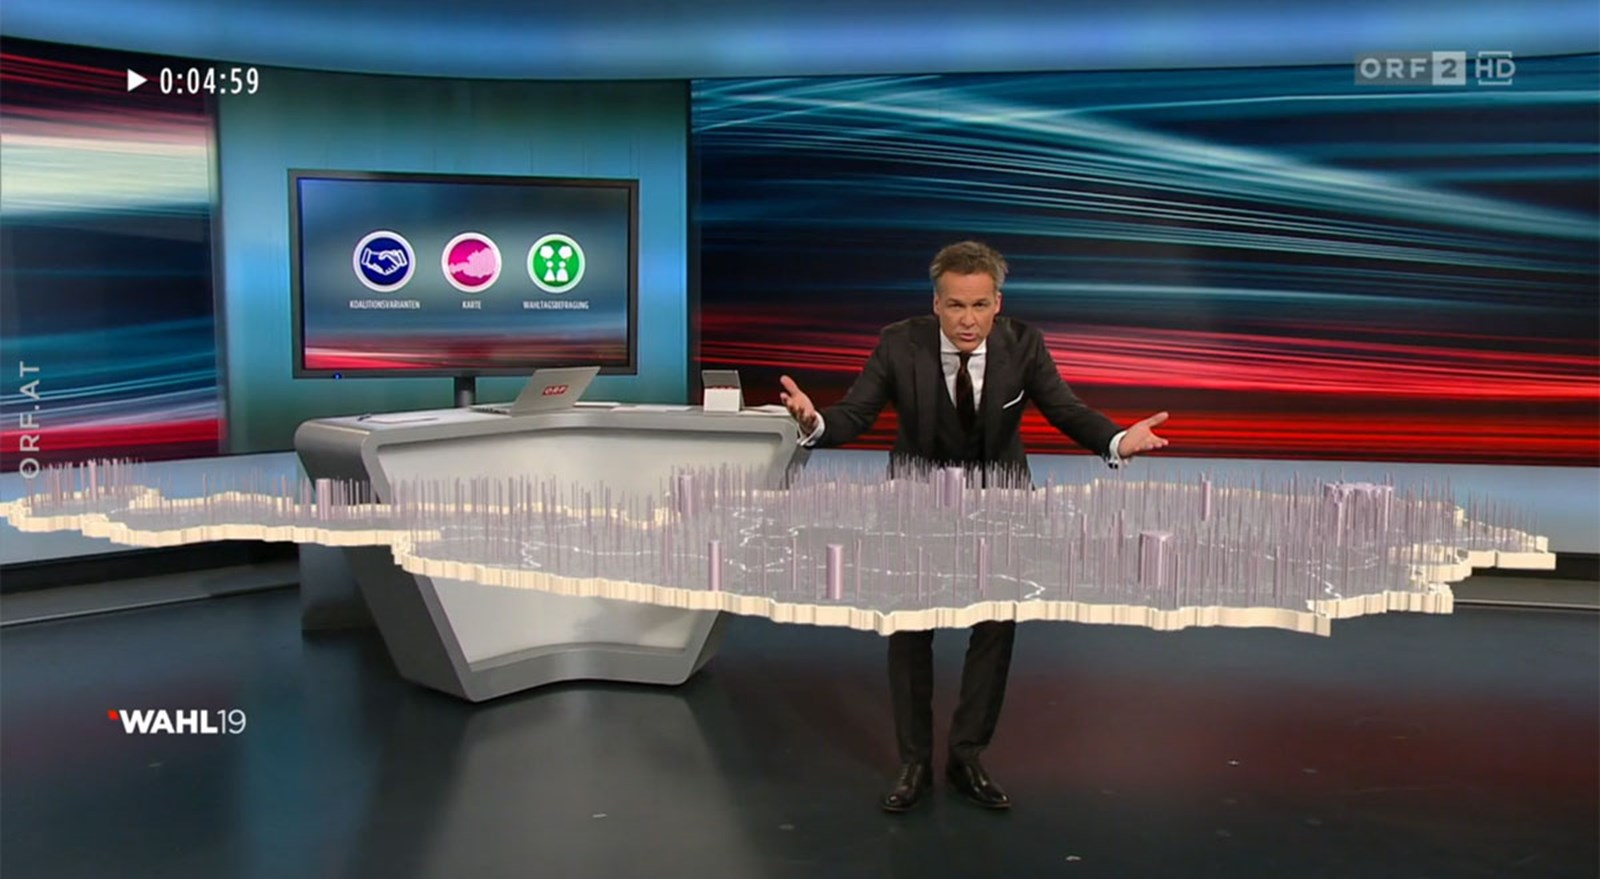
\includegraphics[width=0.78\textwidth]{media/election.jpg}
		\hfill
		\caption{Augmented reality showing election results on TV, taken from~\cite{fluch19}.}
		\label{fig:election}
	\end{figure}

	%\begin{figure}[!ht]
	%	\captionsetup{justification=centering}
	%	\centering
	%	\subfloat[{Augmented reality showing election results on TV, taken from~\cite{fluch19}.}]{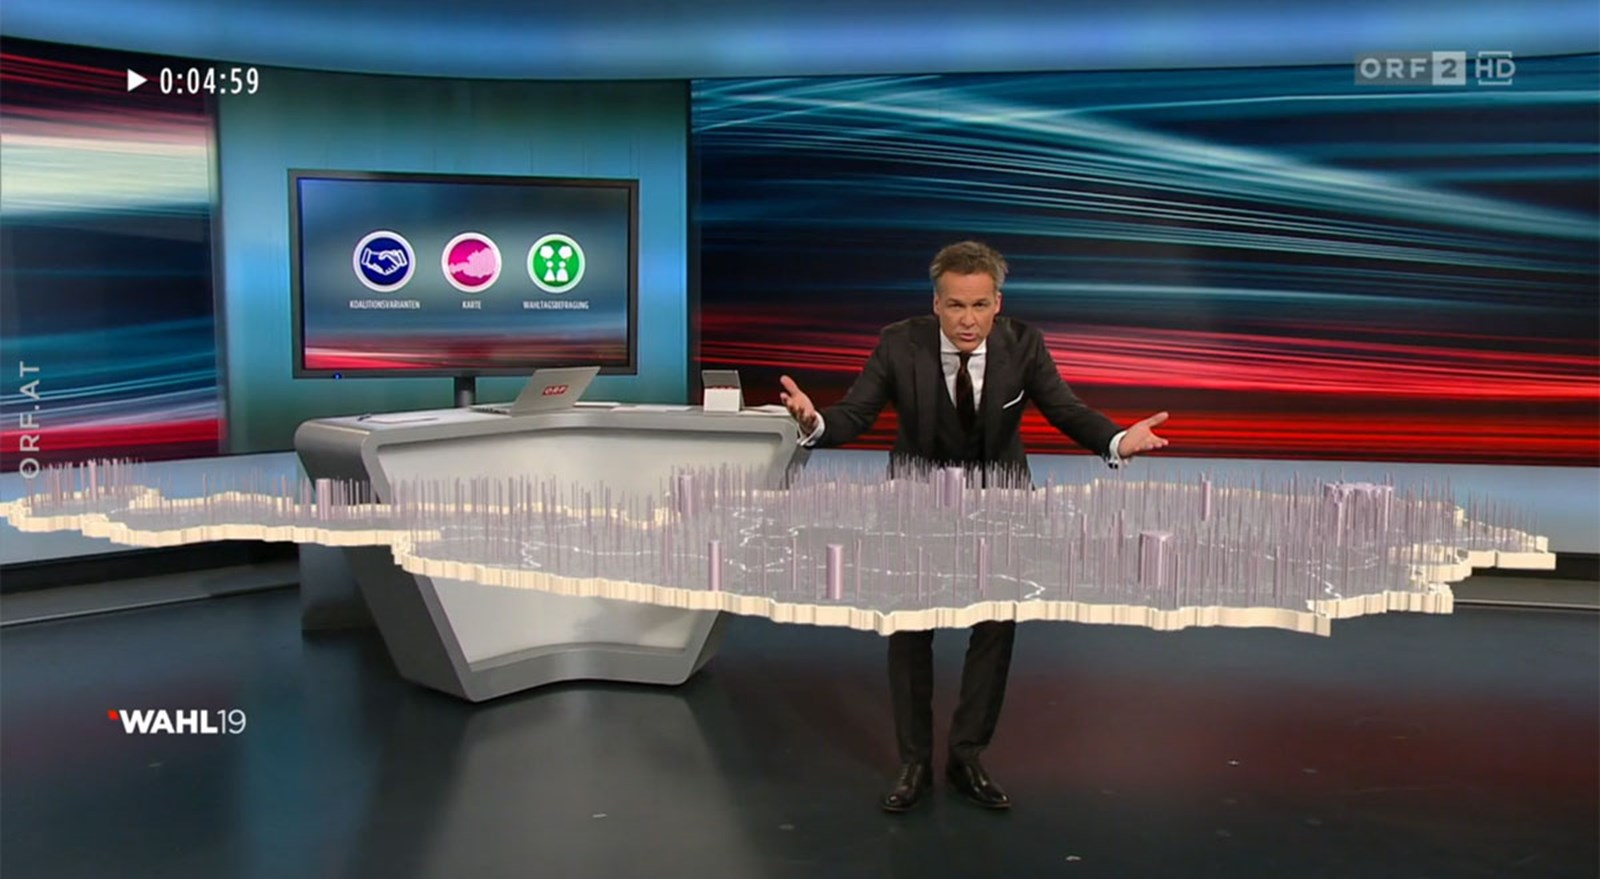
\includegraphics[width=0.47\textwidth]{media/election.jpg}\label{fig:election}}
	%	\hfill
	%	\subfloat[{Flooding in the studio, made possible by IBM Max Reality, taken from~\cite{ibm}.}]{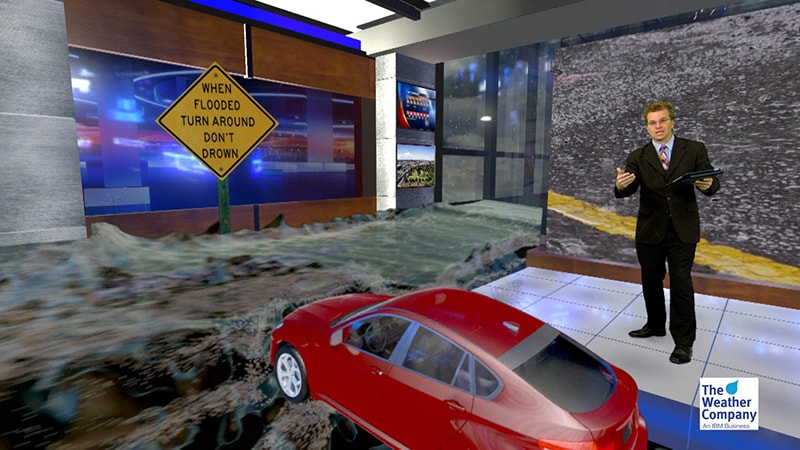
\includegraphics[width=0.47\textwidth]{media/ibm_max_reality.jpg}\label{fig:ibm_mr}}
	%	\hfill
	%	\caption{Preview scaling of two different sized models.}
	%	\label{fig:tv_ar}
	%\end{figure}
	
\end{description}